\documentclass[a4paper]{article}
\usepackage{ctex}
\usepackage{enumitem}
\usepackage{multirow}
\usepackage{fancyhdr}
\usepackage{amsmath}
\usepackage{parskip}
\usepackage{float}
\usepackage{hyperref}

\setlength{\parskip}{6pt}

\pagestyle{headings}

\begin{document}
\title{课程设计:图片搜索引擎}
\author{梁业升 2019010547(计03)}

\maketitle

\section{问题描述}\label{sec:problem}

实现一个图片搜索引擎,支持通过图片搜索相近图片、筛选尺寸和颜色等功能。

使用的数据集为 \hyperlink{Google Landmark Retrieval 2019}{https://www.kaggle.com/competitions/landmark-retrieval-2019/overview}。此
数据集为景点图片,其目的是实现通过景点的图片检索对应的景点。

本项目的目标包括:

\begin{itemize}
    \item 能够通过原图搜索到正确的图片
    \item 能够通过略有改动的图片搜索到正确的图片
    \item 能够通过相同景点的不同图片搜索到正确的景点
    \item 支持筛选尺寸和颜色
\end{itemize}

\section{实现模块}

项目分为四个部分:

\begin{description}
    \item[后端] 处理图片索引、执行图片搜索。HTTP 框架为 Flask,图片处理与相关计算使用 OpenCV、Numpy 和 Scipy。
    \item[前端] 上传图片、设置规则、显示结果。使用 React 和 Chakra-ui 实现 UI。
    \item[数据库] 主数据库为 Sqlite,使用 Redis 进行缓存。
    \item[下载器] 并行下载数据集中的图片文件,使用 Go 实现。
\end{description}

\section{关键功能}

\subsection{索引结构}

图片关系定义如下:

\begin{description}
    \item[\texttt{id}] 自增主键,整数
    \item[\texttt{file\_name}] 图片文件名,字符串
    \item[\texttt{features}] 图片特征,向量(以字符串存储)
    \item[\texttt{distance}] 图片特征与某一标准特征的距离,浮点数
    \item[\texttt{colors}] 图片的主要颜色,向量(以字符串存储)
    \item[\texttt{width}] 图片宽度,整数
    \item[\texttt{height}] 图片高度,整数
\end{description}

关于特征和距离的定义,详见 \ref{sec:feature-extraction} 和 \ref{sec:distance-calculation}。

\subsection{特征提取}\label{sec:feature-extraction}

此部分内容参考了 \hyperlink{image-search-engine}{https://github.com/kudeh/image-search-engine} 的实现,
对应 \texttt{backend/app/utils.py} 中的 \texttt{ColorDescriptor} 类。

首先,将图片转换为 HSV 色彩空间,并将图片分为左上、右上、左下、右下四个长方形区域和中间的椭圆形区域。
对于每个区域,使用 OpenCV 的 \texttt{calcHist} 函数生成图片直方图(Image Histogram,即区域内的亮度分布)。
将直方图进行正规化,并将五个区域的直方图拼接成一个向量,即为图片的特征。

\subsection{距离计算}\label{sec:distance-calculation}

计算两个图片通过 \ref{sec:feature-extraction} 的方法提取的特征向量之间的卡方距离(Chi-Squared Distance)。定义此
距离为两个图片之间的距离;距离越小,两个图片相似程度越高。

同时,定义“标准距离”为图片特征向量与全 0 向量的卡方距离(即特征向量和的一半)。在建立索引时,将此距离存入数据库中。

\subsection{主要颜色提取}

此部分内容参考了 \hyperlink{Dominant-Color-Extraction-Dominance-and-Recoloring}{https://github.com/srijannnd/Dominant-Color-Extraction-Dominance-and-Recoloring}
的实现,对应 \texttt{backend/app/utils.py} 中的\\ \texttt{get\_prominant\_colors} 函数。

对图片的像素进行 k-means clustering 处理,即可得到图片从大到小排序的主要颜色。

\subsection{图片搜索}

图片数据以 base64 编码传输。

后端首先使用图片数据计算图片的特征向量和标准距离。

我们认为,相近的图片其(正规化后)特征向量的和也应当相近,因此我们在查询数据库时只取标准距离和查询图片的标准距离相差在一定
范围内的图片,以节省时间。这种方法有可能导致最后返回的结果中不包含最接近的图片,因此需要仔细选取范围。

在使用上面方法获得索引内的若干图片后,我们逐一计算图片与查询图片的距离,并根据距离进行排序。

然后,我们将这些结果使用图片数据的 MD5 值作为键缓存到 Redis 中,这样在重复查询相同图片时无需再次计算。

最后,对上面的结果进行宽度、高度和颜色的筛选。其中颜色筛选的方法为比较查询图片和结果图片的主要颜色之间的 RGB(欧氏)距离,若
距离相近,则保留此结果,否则不返回。筛选结束后,返回结果。

\section{测试结果和样例分析}

我们对 \ref{sec:problem} 中提出的的目标进行测试和分析:

\begin{itemize}
    \item 能够通过原图搜索到正确的图片
    \item 能够通过略有改动的图片搜索到正确的图片
    \item 能够通过相同景点的不同图片搜索到正确的景点
\end{itemize}

由于算法是确定的,因此相同图片之间的距离一定是 0,在索引正确的情况下能够保证一定能够搜到,因此省略此部分的测试。

\subsection{略有改动的图片}

我们对原图分别进行遮挡、曝光度和色温调整、裁剪操作,测试搜索的结果。其中最左侧的图片为查询图片,右侧分别为返回
的第一、第二个结果,其数值为与查询图片的距离。

\subsubsection{遮挡}

\begin{figure}[H]
    \centering
    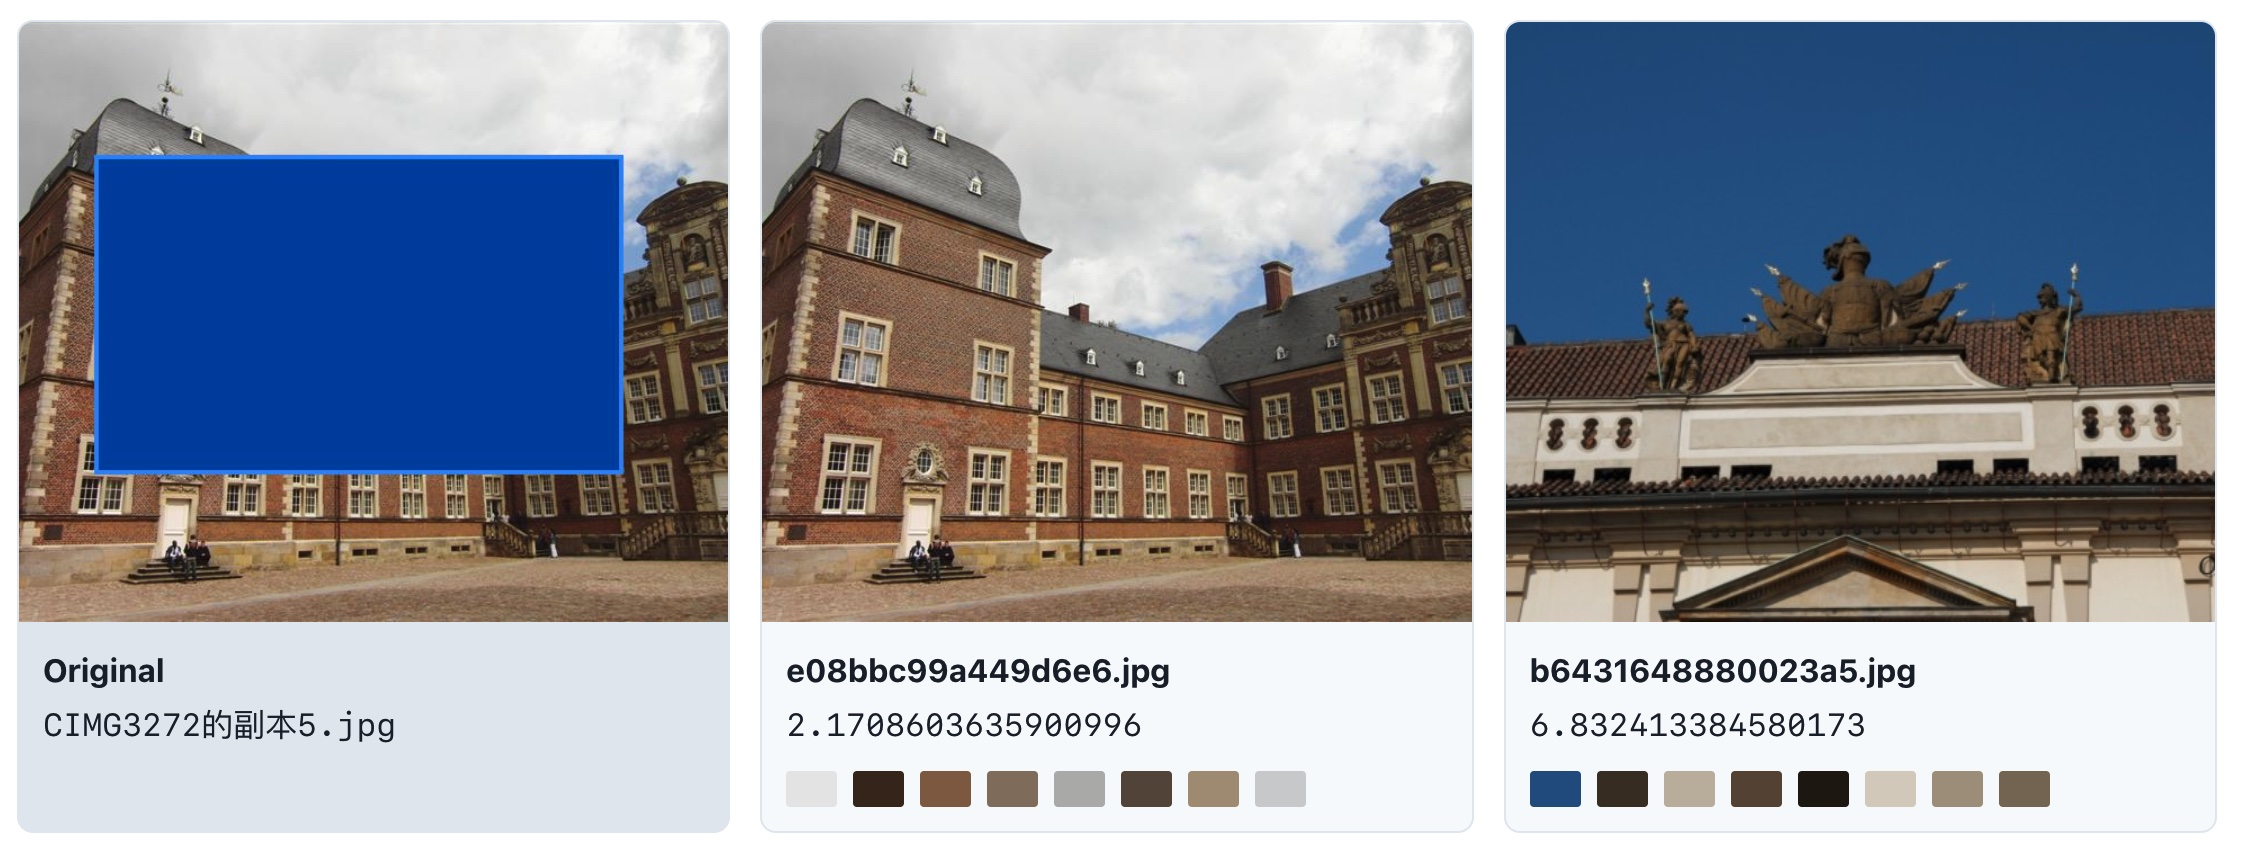
\includegraphics[width=\textwidth]{assets/test-1-1.jpg}
    \caption{遮挡部分区域}
    \label{fig:search_result_1_1}
\end{figure}

\begin{figure}[H]
    \centering
    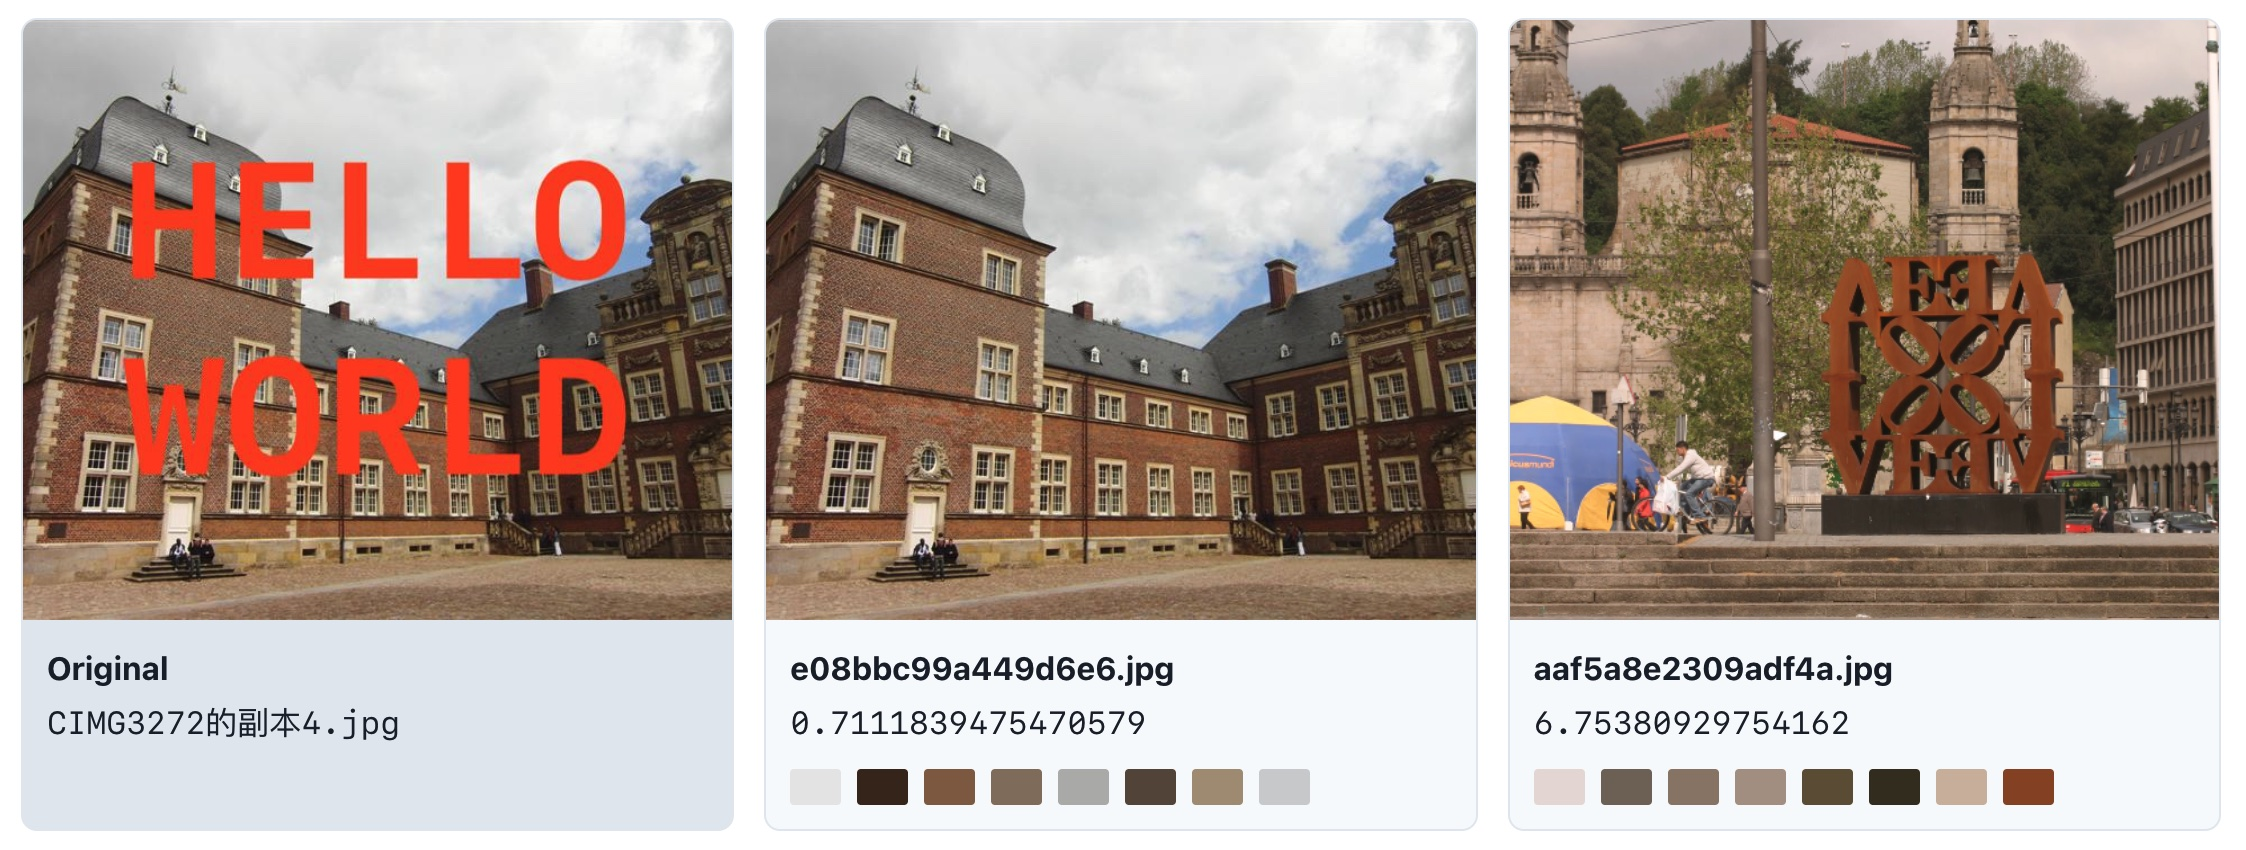
\includegraphics[width=\textwidth]{assets/test-1-2.jpg}
    \caption{文字遮挡}
    \label{fig:search_result_1_2}
\end{figure}

可以看到,尽管进行了较大的遮挡,搜索引擎仍然能够返回正确的结果,可见通过分别对五个区域进行特征提取有不错的效果。

\subsection{对比度和色温调整}

调整原图的对比度和色温进行测试:

\begin{figure}[H]
    \centering
    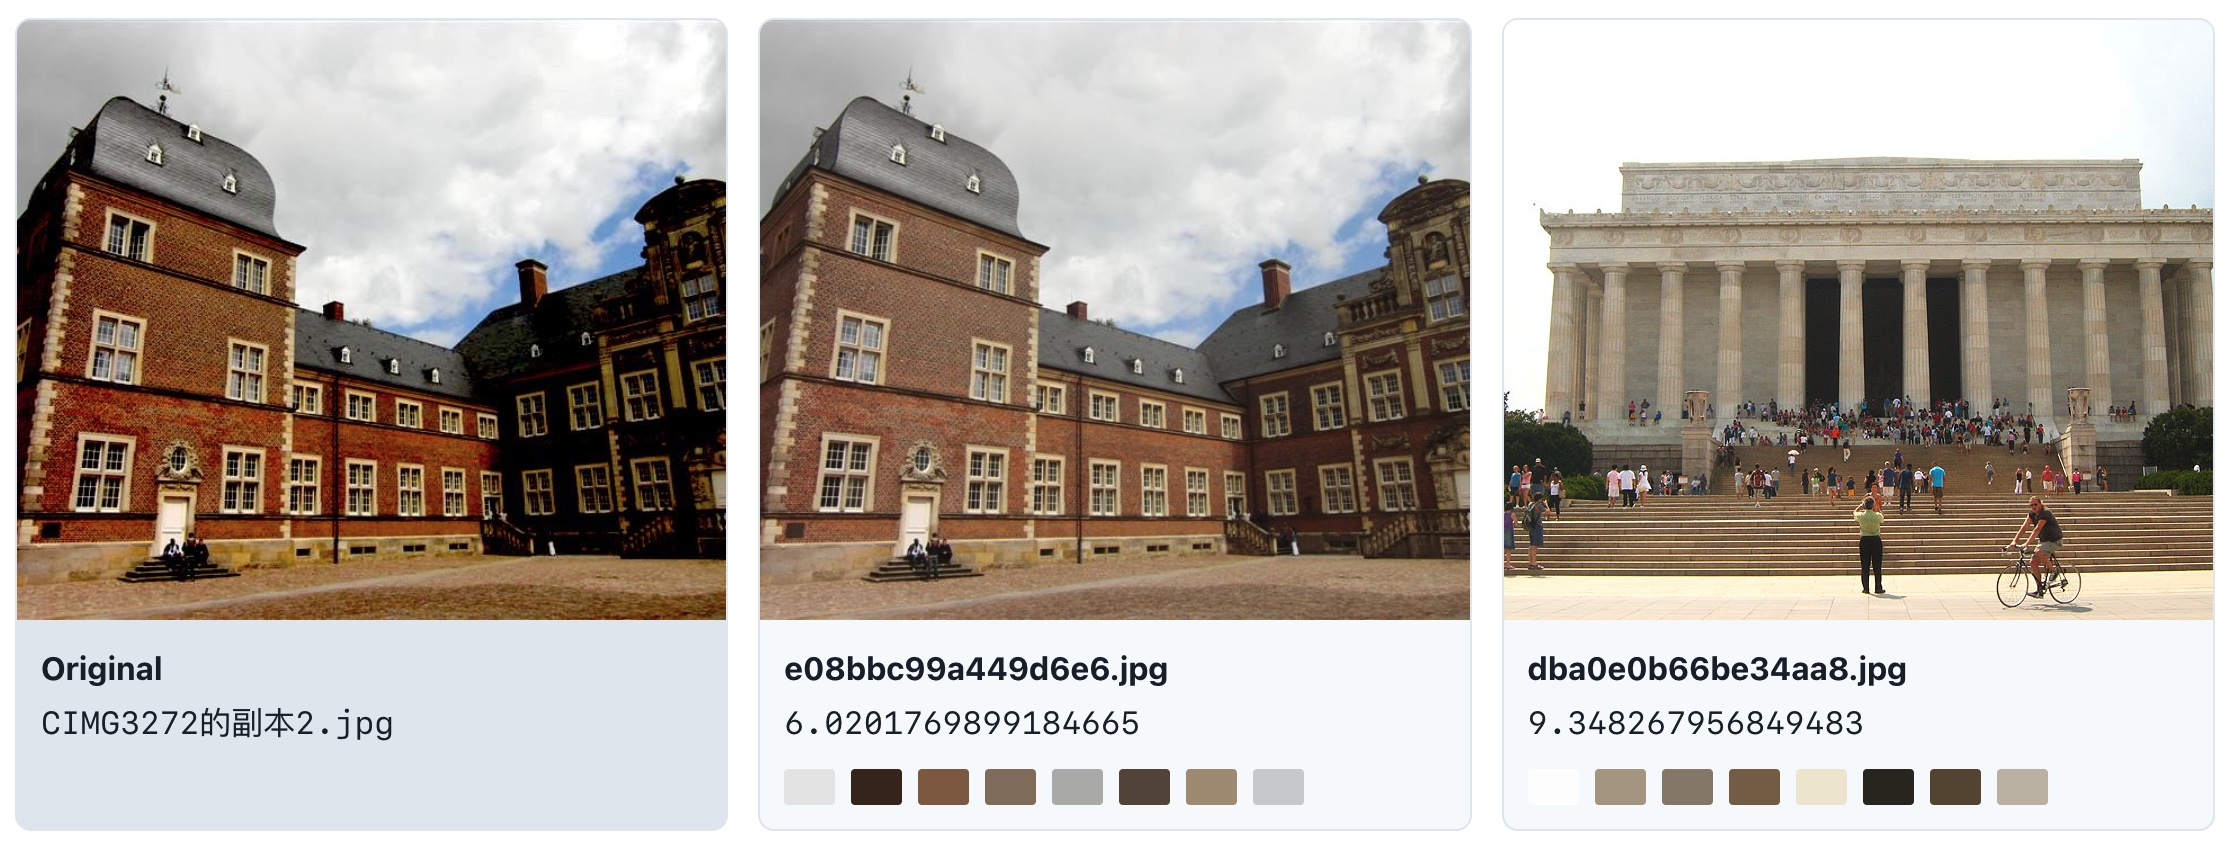
\includegraphics[width=\textwidth]{assets/test-1-3.jpg}
    \caption{对比度和色温调整}
    \label{fig:search_result_1_3}
\end{figure}

可以看到,搜索引擎仍然返回正确的结果,不过其准确率有所下降(距离较大),只能应对一定程度内的调整。

\subsubsection{裁剪}

\begin{figure}[H]
    \centering
    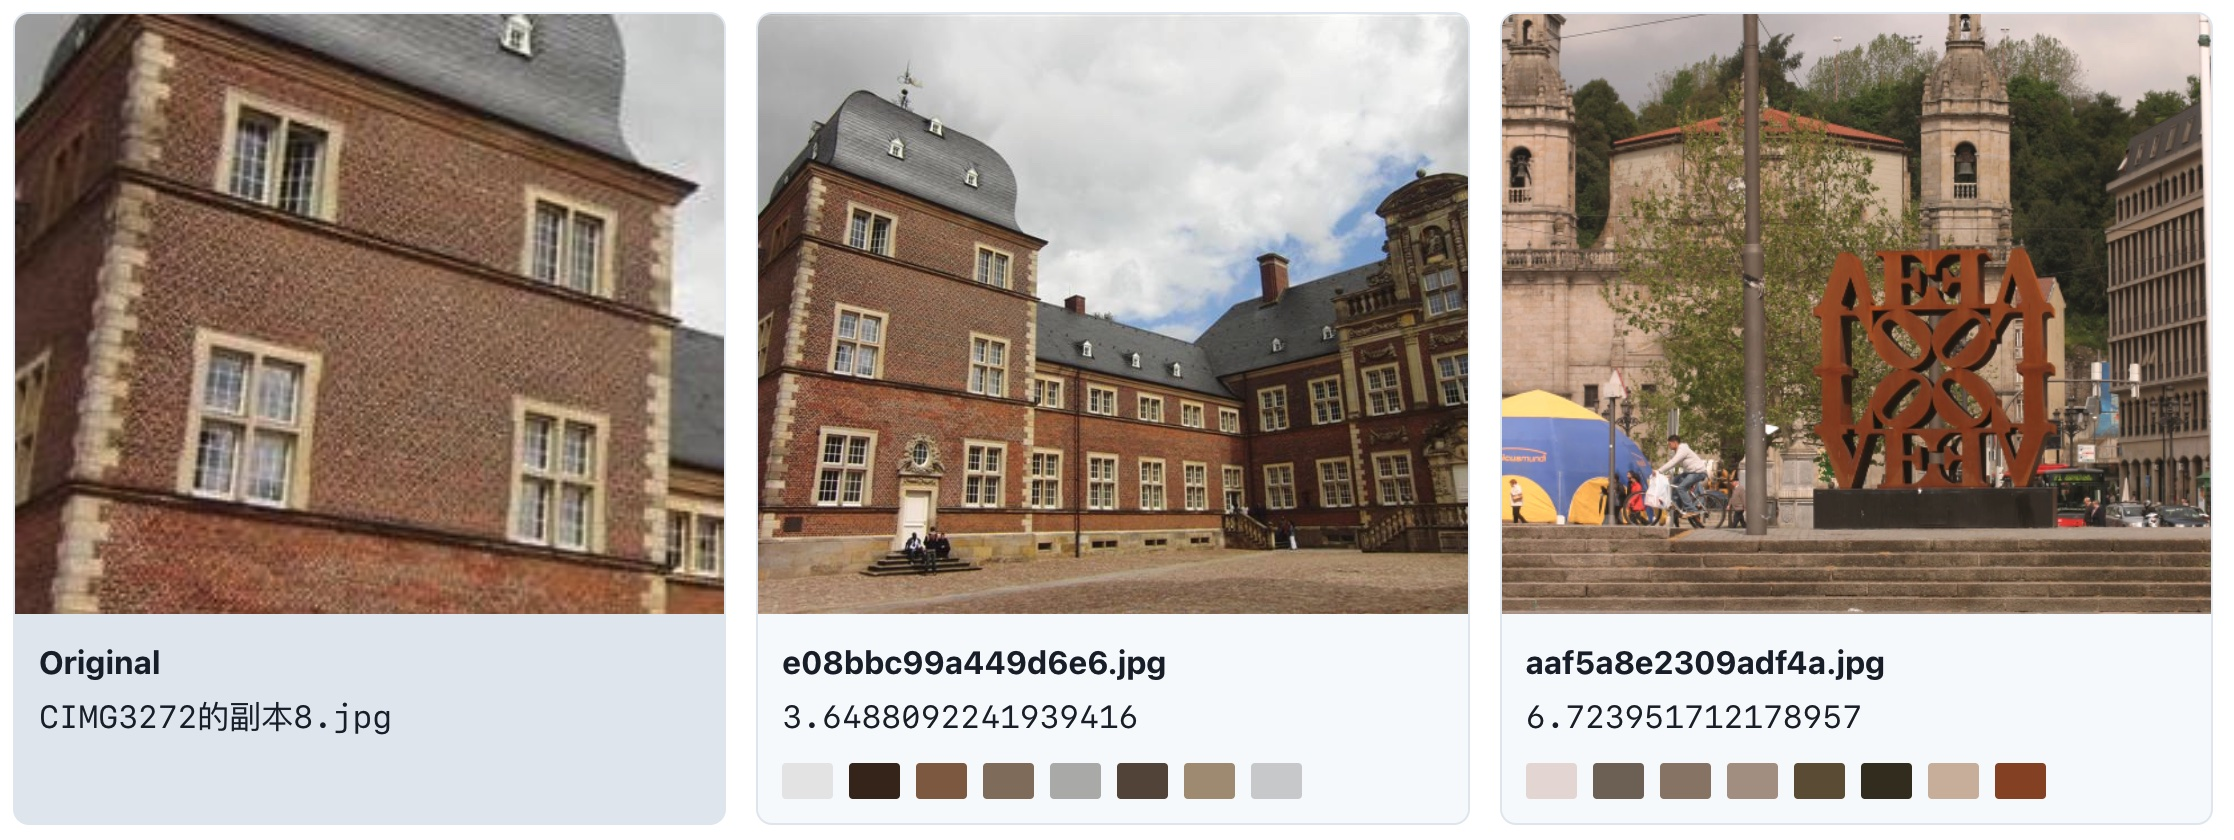
\includegraphics[width=\textwidth]{assets/test-1-4.jpg}
    \caption{裁剪}
    \label{fig:search_result_1_4}
\end{figure}

我们只保留建筑的主要部分进行搜索,搜索引擎能够返回正确的结果,而且效果不错(距离较小)。

\subsection{另外角度的图片}

我们使用同一地点的不同照片进行搜索。

\begin{figure}[H]
    \centering
    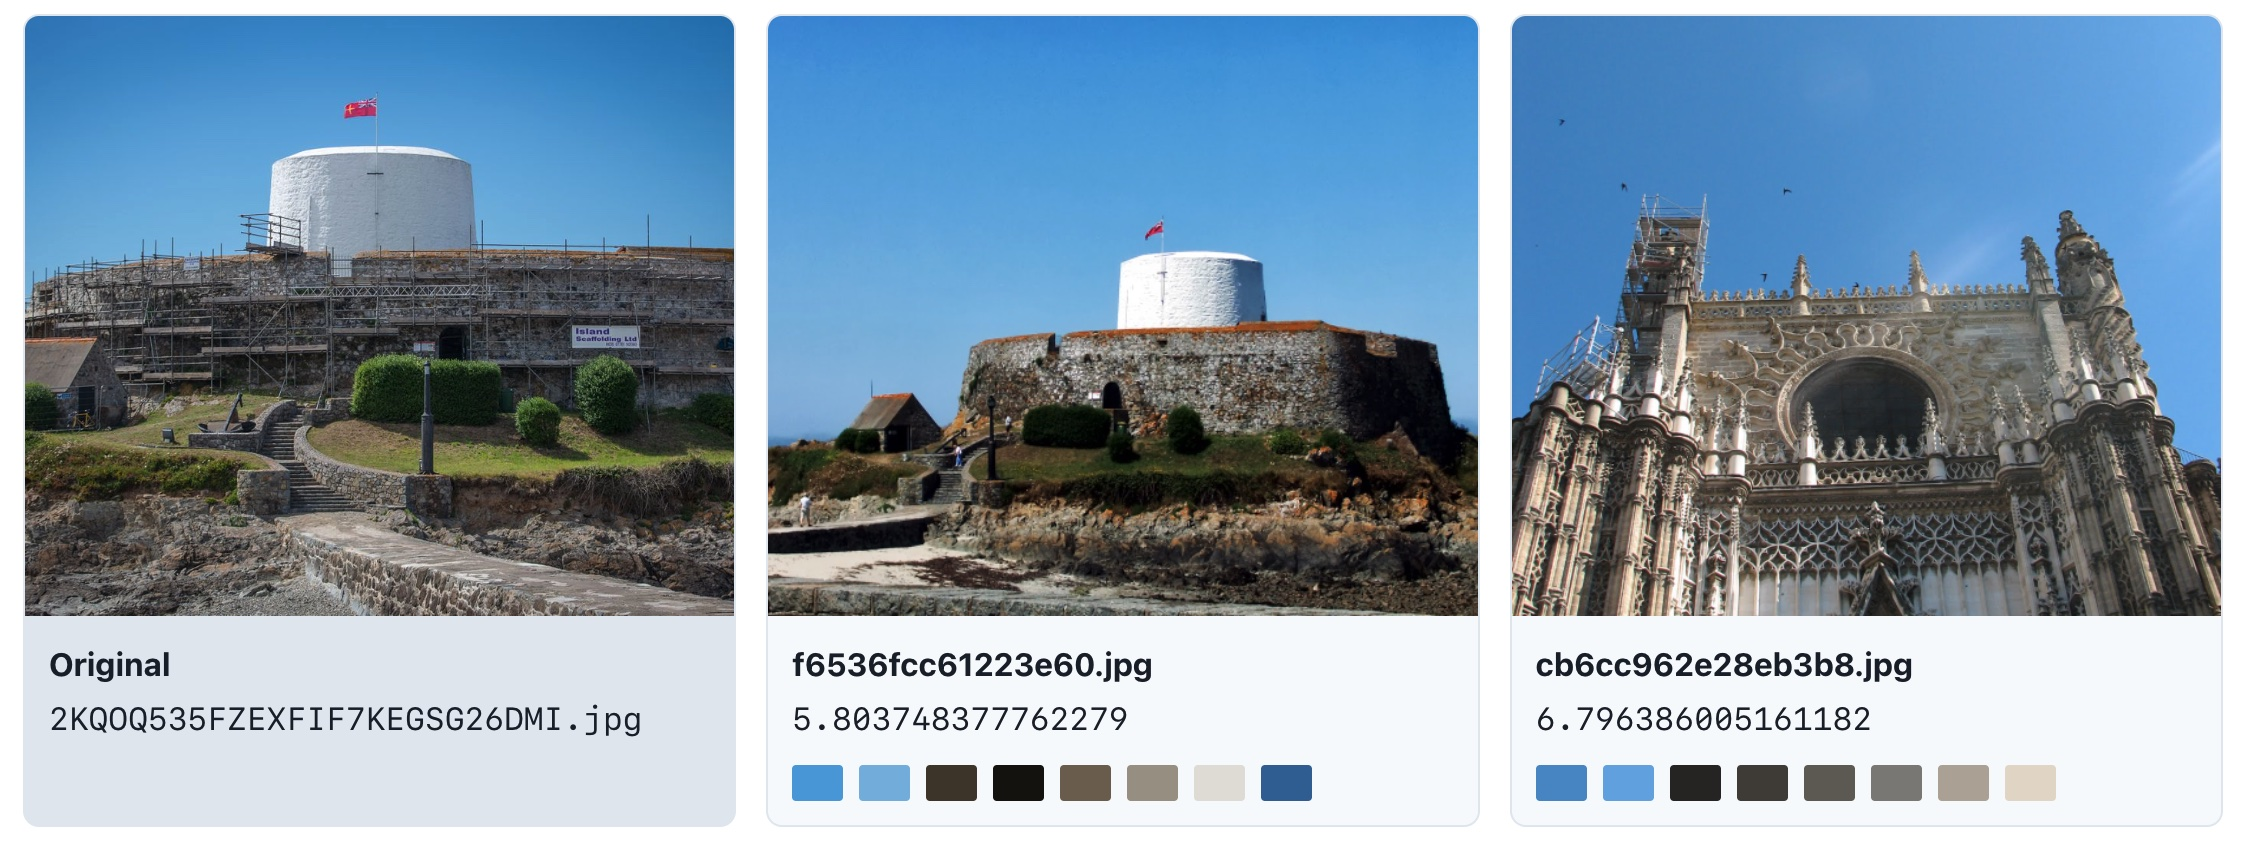
\includegraphics[width=\textwidth]{assets/test-2-1.jpg}
    \caption{成功例子-1}
    \label{fig:search_result_2_1}
\end{figure}

\begin{figure}[H]
    \centering
    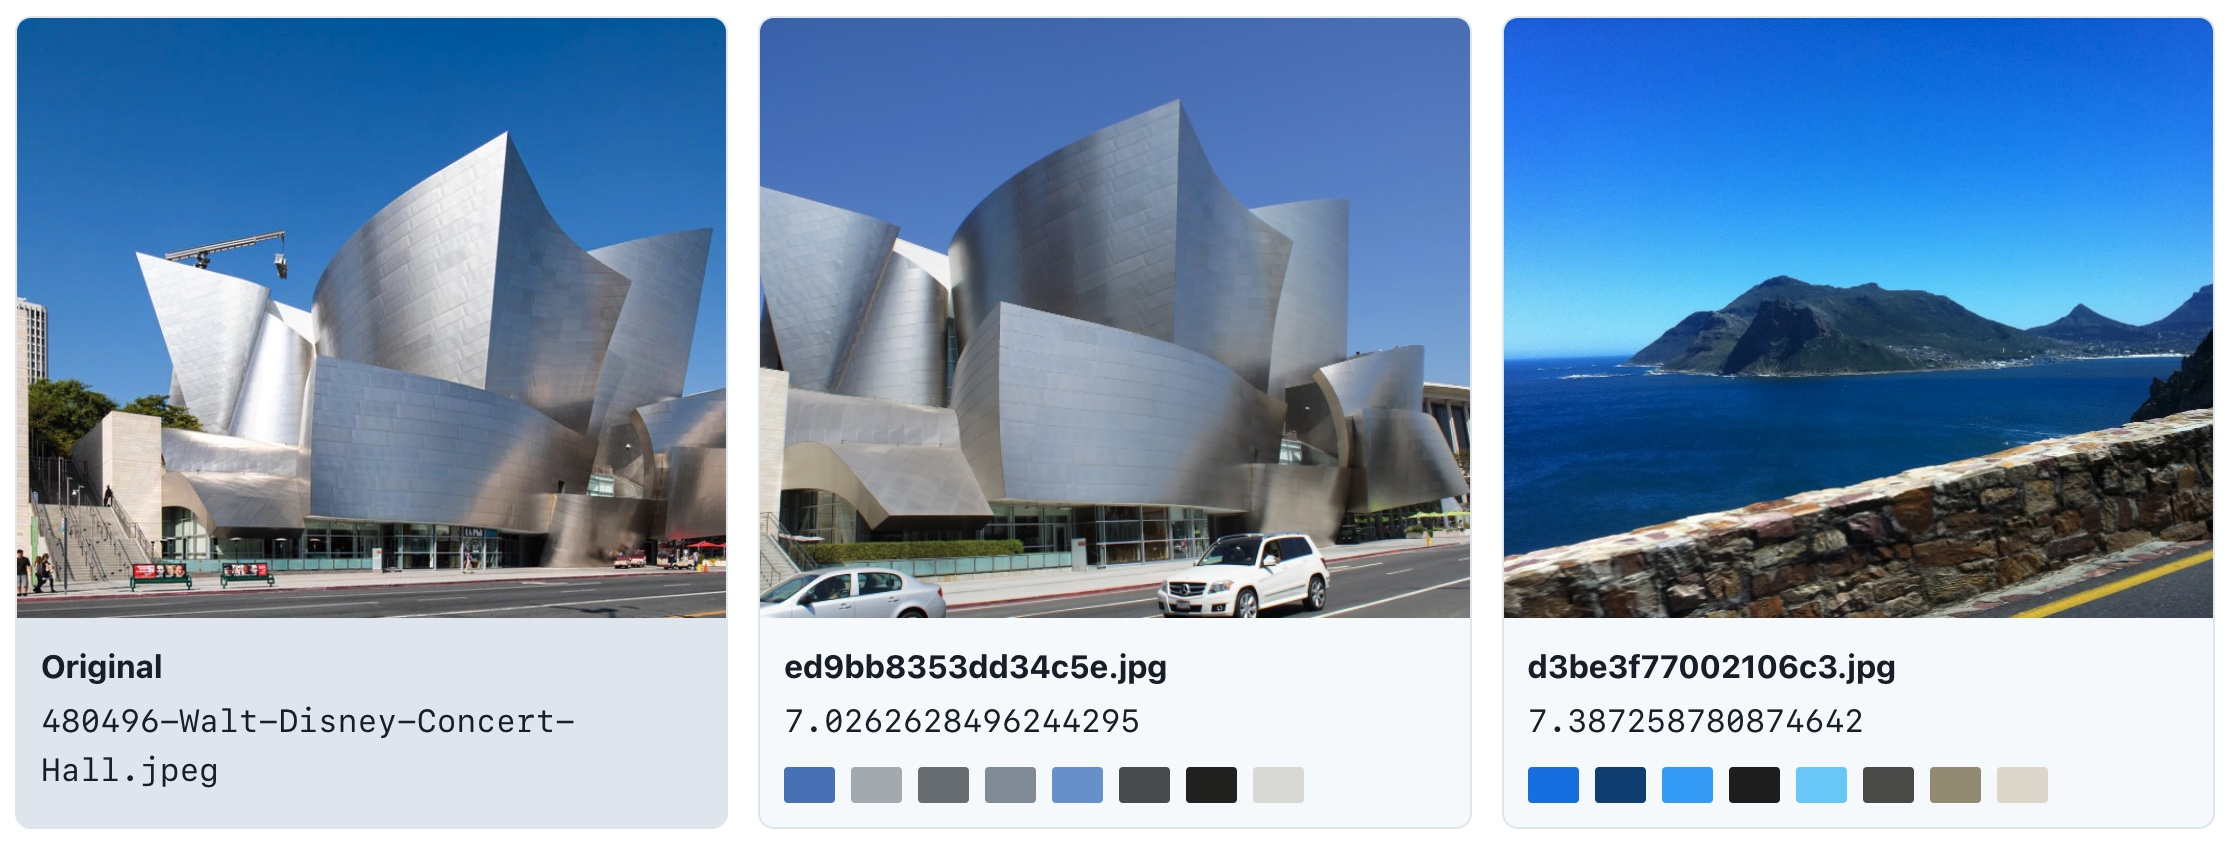
\includegraphics[width=\textwidth]{assets/test-2-2.jpg}
    \caption{成功例子-2}
    \label{fig:search_result_2_2}
\end{figure}

可以看到,对于同一个地点的不同照片,在相似度较高的情况下,搜索引擎能够正确返回对应的景点。值得注意的是,背景颜色对
搜索结果的影响较大:在第二个例子中,天空的颜色差别相对较大,导致图片的距离较大。这个问题可以通过缩小图片的有效范围
来改善。

\begin{figure}[H]
    \centering
    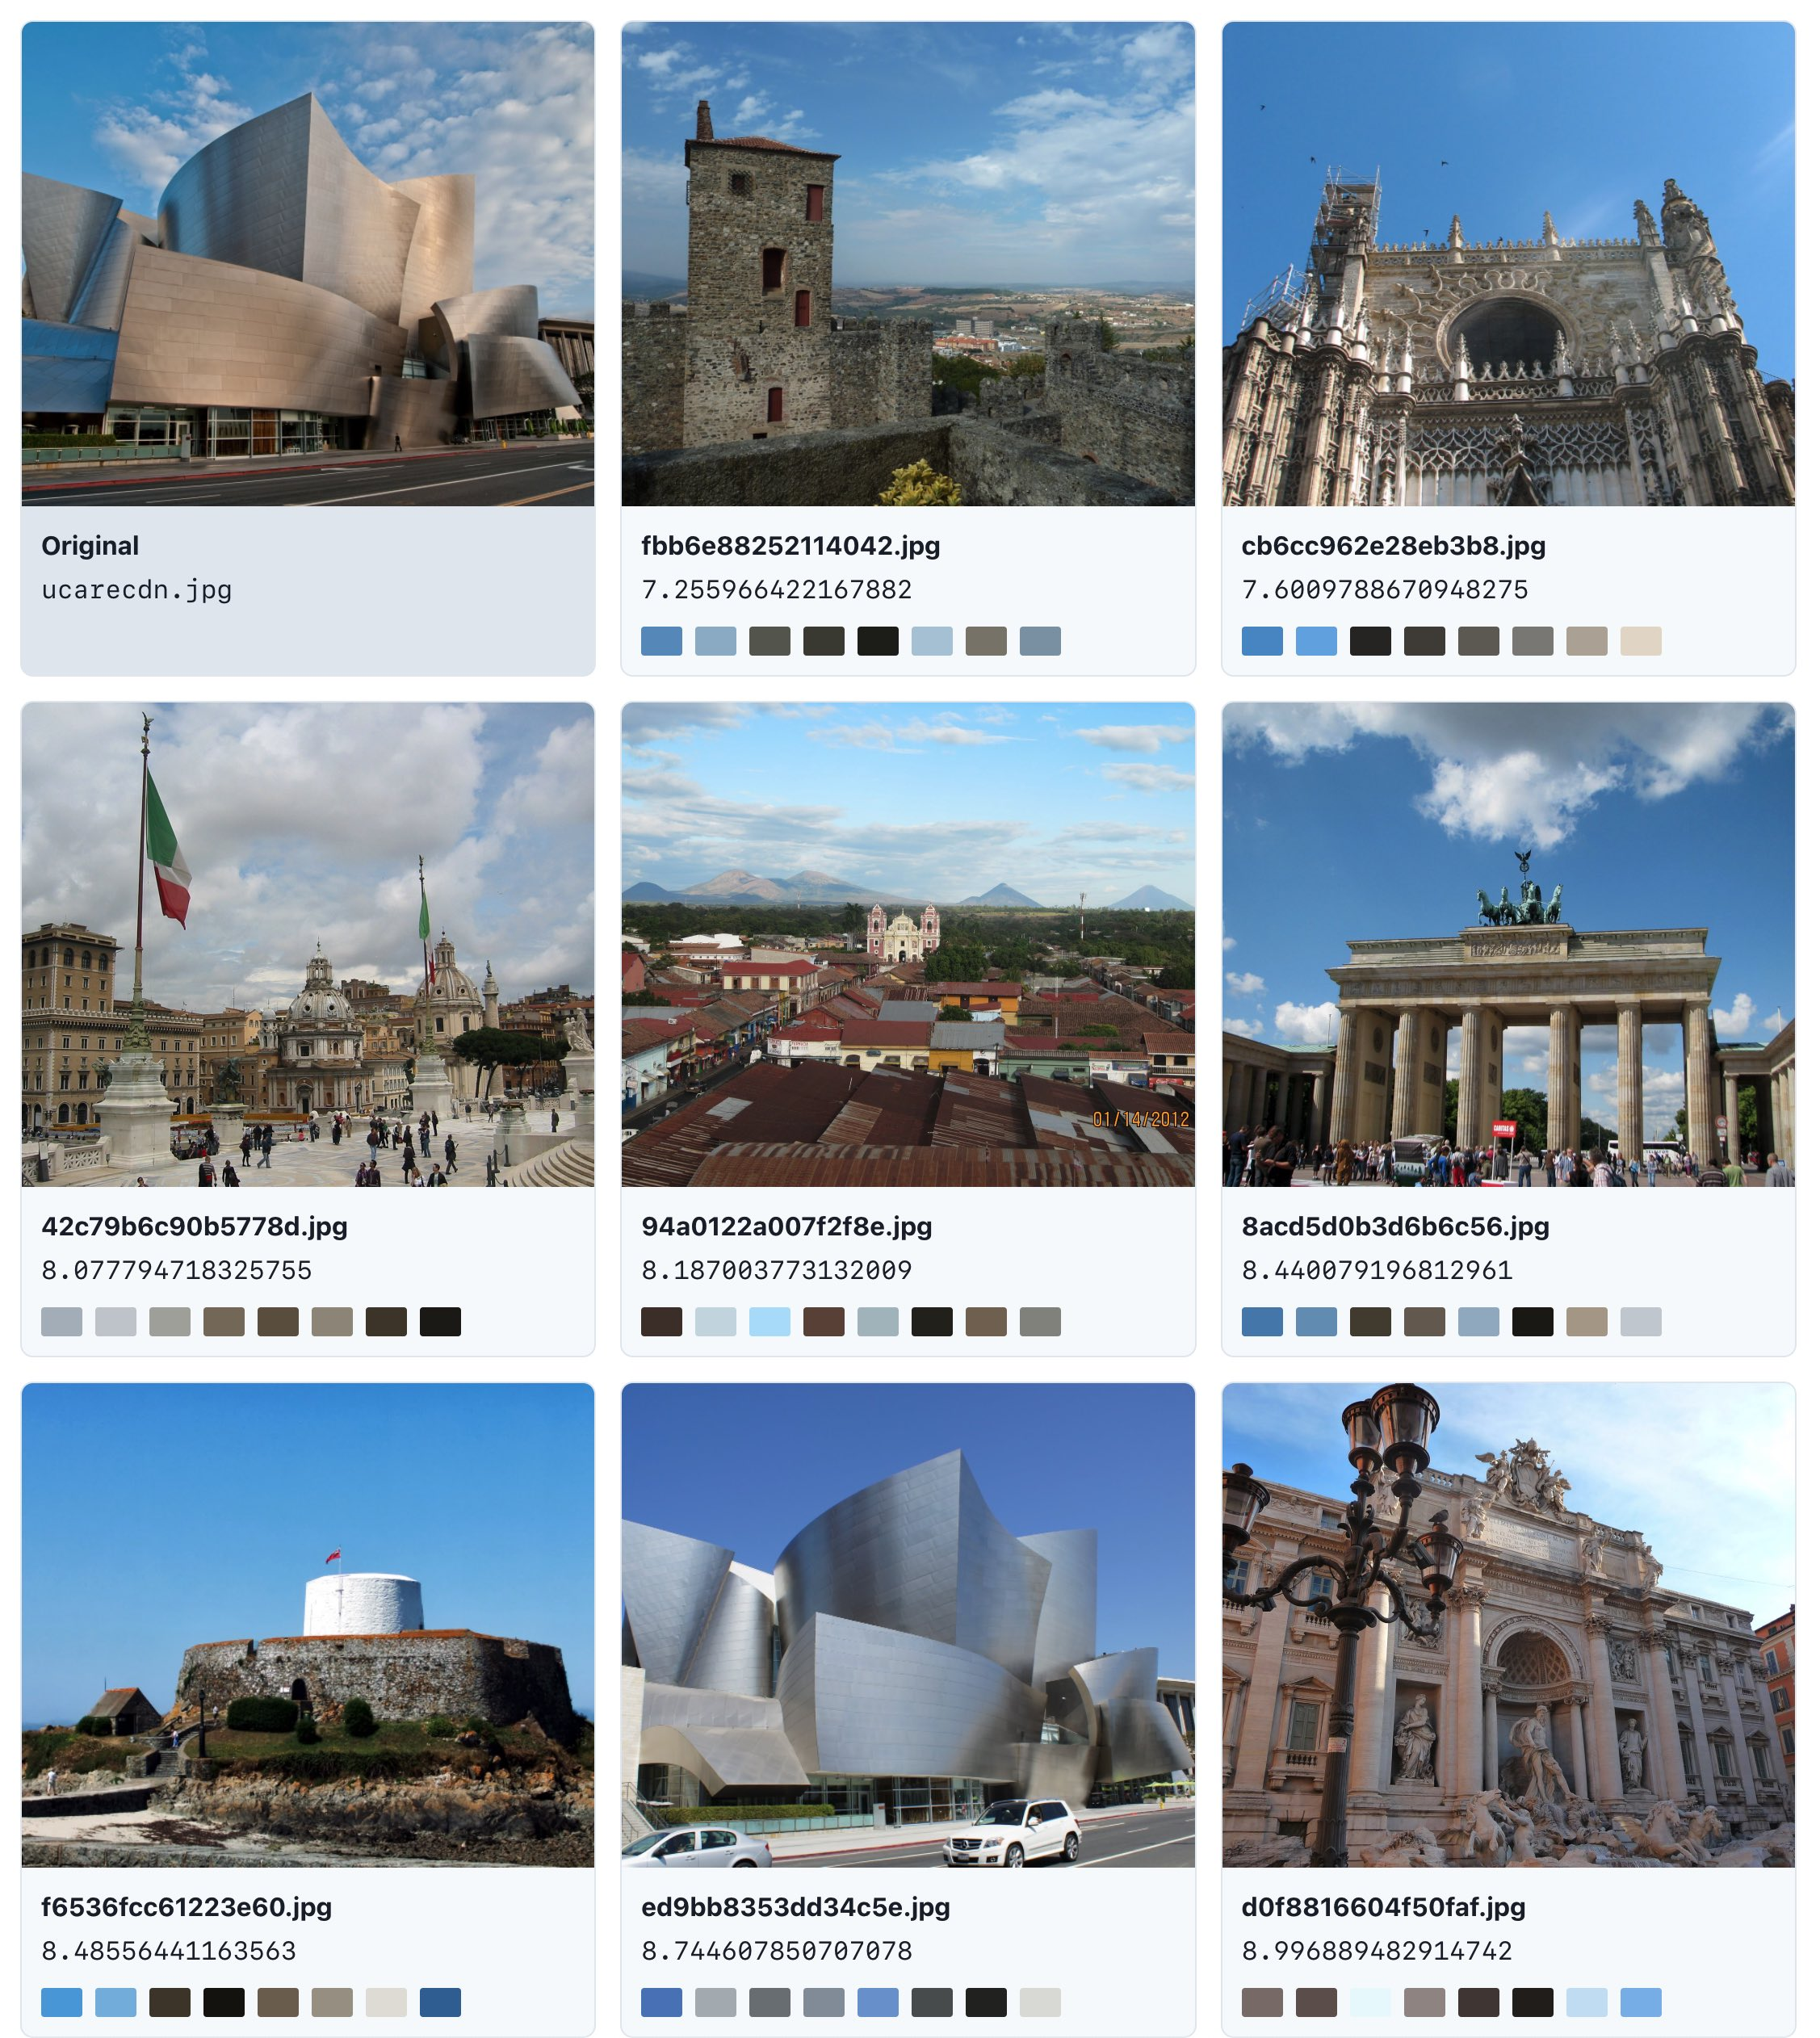
\includegraphics[width=\textwidth]{assets/test-2-3.jpg}
    \caption{失败例子}
    \label{fig:search_result_2_3}
\end{figure}

这个例子是个典型的失败例子。虽然建筑物是相同的,但由于光照不同其颜色不同,导致正确的结果在仅排在第 7。

这也是使用相似度进行景点匹配的局限性:仅仅考虑图片之间的相似程度,而对图片的语义没有任何的了解。通过结
合物体识别算法,应该能够在较大程度上改善这个问题。

\section{参考资料}

特征提取:\hyperlink{image-search-engine}{https://github.com/kudeh/image-search-engine}

颜色提取:\hyperlink{Dominant-Color-Extraction-Dominance-and-Recoloring}{https://github.com/srijannnd/Dominant-Color-Extraction-Dominance-and-Recoloring}

\end{document}
